\subsection{Class Diagram}
This section will explain the most notable classes illustrated in \cref{fig:class}, their relations and their motivation and responsibilities.

\subsubsection{Coordinate}
The \emph{Coordinate} trait models a geographic location on the earth. Because many functions are dealing with objects that can have coordinates, we can let these objects implement the \emph{Coordinate} trait, and thereby write these functions in a polymorphic way. One such object is the \emph{Position} class, which is essentially a coordinate for a person at a given time.

\emph{ConfidencePosition} is designed to have the same structure as positions received from the aSTEP server, so when our application requests position data, a list of \emph{ConfidencePosition} will be returned. A \emph{ConfidencePosition} therefore also includes information about the certainty of a position, called \emph{Confidence} as shown on \cref{fig:class}. This confidence denotes a square around the observation that has a 95\% chance to include the observed unit\cite{cisco}. \emph{ConfidencePosition} also has a \emph{lastLocatedTime} which is a time stamp for when the position was recorded by the aSTEP server.

\subsubsection{Person}
The \emph{Person} class is an abstract class, defining methods which should be implemented in specialisations of this class, in order to enforce code reuse and consistency. The class contains the person's history of positions as an iterable collection of the generic type \emph{T}. 

The generic type parameter \emph{T} is bounded to be a class implementing \emph{Coordinate}, denoted by \emph{T < Coordinate}. This prevents any specialisation of \emph{Person} from having a history of positions that is not a collection of \emph{Coordinate}s. \emph{T} is in a contravariant position, denoted by \emph{-T}, permitting specialisations of the \emph{Person} class to use a specialisation of \emph{T}. Contravariance allows the \emph{Person} class to have methods that takes an input of type \emph{T}, but excludes the class from defining methods which returns a \emph{T}. 

The most important method in the \emph{Person} class is \emph{movePerson}, which takes a \emph{T} and a \emph{DateTime} as parameters. Here the parameter of type \emph{T} is the location the person should be moved to, and the DateTime parameter is the time where the person arrived at the location. This method updates a person's history of positions to include the new position. Upon updating a person's history of positions, positions older than \emph{x} is removed from the person, where \emph{x} is a constant defined for all persons. To calculate a person's velocity and heading direction this history of positions is essential.

\emph{FakePerson} is a concrete class inhering from \emph{Person[Position]}, which has a iterable collection of \emph{Position}s. \emph{FakePerson}s are used for simulations with generated position data. When dealing with \emph{FakePerson} we found it necessary to have an id in the \emph{Position} class in order to implement the \emph{movePerson} method for \emph{FakePerson}, which is why a \emph{Coordinate} were insufficient. 

When positions from the aSTEP core are used we keep confidence information in case it would be useful at some point. This is why a \emph{RealPerson} inherits from \emph{Person[ConfidencePosition]}.

\subsubsection{Area}
\emph{Area} is an abstract class representing a geographical area on a map. The most important method in the class that should implement is the function \emph{isWithinArea}. There are two versions of the function. One takes a coordinate and returns a boolean denoting weather this coordinate is within the area. The other takes a iterable collection of generic types T and a function that goes from T to a coordinate. It returns a new filtered iterable collection of T only consisting of the objects within the area.

\subsubsection{PopulatedArea and Population}
\emph{PopulatedArea} is a class mixing an \emph{area} with \emph{population}. The \emph{population} is responsible of caching and updating the positions of people. The \emph{PopulatedArea} is then responsible of combining the population with the area, making sure that the \emph{Population} is only populated with positions within the area. The two main things the \emph{Population} must be able to do, is to update the positions of the people and be able to find the positions of all the people given a time. Since the \emph{Population} is responsible for caching of peoples positions it also hold the policy of when to throw away positions and to extension the people holding them, if they for instance leave the area and the \emph{PopulationArea} no more provide positions, making the person irrelevant. The \emph{Population} is therefore also responsible for any misses in its people position cache, and request the aSTEP for these positions. Since it is people themselves that throw away their positions the \emph{Population} class must know about the policy of the person given to it, in order to be able to know when to request new positions from the aSTEP core and add these to the person. \emph{Population}, together with the \emph{Person} class, hold the policy on how to, given a specific time stamp, find the position closest to this time stamp for each person, and judging when there is one close enough.

\subsubsection{AnalyserData}
\emph{AnalyserData} is the class holding the information about a person needed by the analyser. Since we wanted the analyser be unaware of the concept of time and in order to simplify the task of analysis, this class holds the coordinate, velocity, and heading direction of a person. The velocity and heading direction is calculated over time, but giving them directly to the analyser through this class, makes the analyser able to ignore time. This means that the analyser will only get an iterable collection of \emph{AnalyserData} and Points from which it should calculate the local crowd factors. 

\subsubsection{Weight and Point}
After the analyser have calculated the local crowd factors it creates the class \emph{Weight} to store them in. The \emph{Weight}s are specific local crowd factors. Together with a \emph{coordinate} for the position of these local crowd factors we get a \emph{Point}. A \emph{Point} is what the client need to represent the local crowd factors to the user. As explained in \cref{subsec:lightweightResults} we do not need to send all local crowd factors as \emph{point}s, but only the top left one as a reference, the resolution, width and hight of the grid and the rest as weights. This way the client can recalculate the positions for the local crowd factors and plot them from the values given in the weights.

\alnote{Person[Position] og Person[ConfidencePosition] skal være abstract, og generalt check diagram}
\begin{sidewaysfigure}[htbp]
\centering
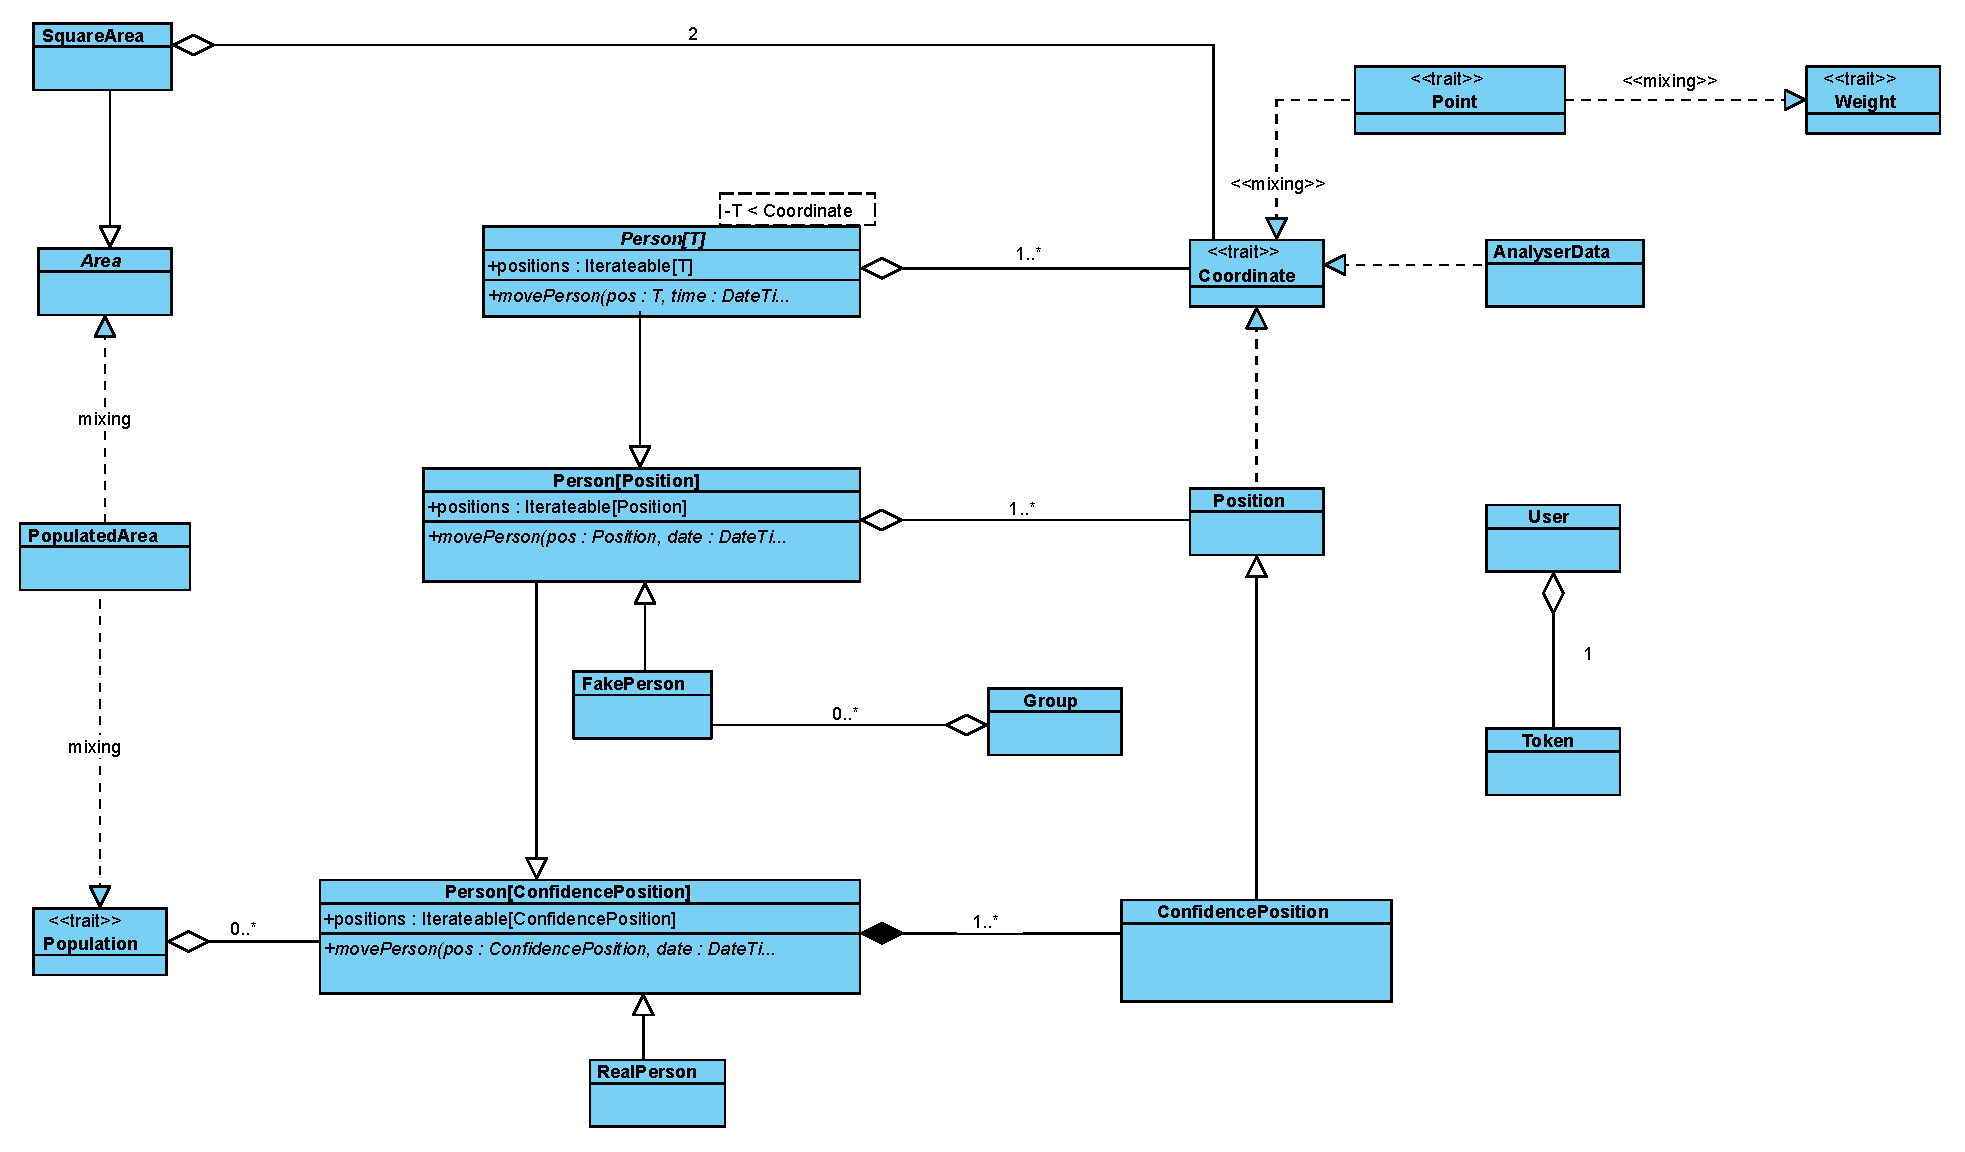
\includegraphics[width=\linewidth]{figures/class.eps}
\caption{Class diagram.}
\label{fig:class}
\end{sidewaysfigure}
